\documentclass[preprint,authoryear,12pt]{elsarticle}

\usepackage{graphicx}
\usepackage{color}
\usepackage{natbib}
\usepackage{amssymb}
\usepackage{amsmath}
\usepackage{amsbsy}
\usepackage{rotating}
\usepackage{gensymb}
%\usepackage{epstopdf}

%Our nomenclature commands
\newcommand{\fmu}{\ensuremath{\mu}}                    %Floquet multiplier
\newcommand{\Ufree}{\ensuremath{\mathrm{U}}}                    %Freestream velocity
\newcommand{\diam}{\ensuremath{\mathrm{d}}}                     %Cylinder diameter
\newcommand{\kinvis}{\ensuremath{\nu}}                 %Kinematic viscosity
\newcommand{\karman}{\mbox{K\'{a}rm\'{a}n}}
\newcommand{\benard}{\mbox{B\'{e}nard}}

%Commands added by us:
\makeatletter
\newcommand{\rmnum}[1]{\romannumeral #1}
\newcommand{\Rmnum}[1]{\expandafter\@slowromancap\romannumeral #1@}
\makeatother

\newcommand{\astar}{\ensuremath{\mathrm{A}^{*}}}
\newcommand{\mstar}{\ensuremath{\mathrm{m}^{*}}}
\newcommand{\crad}{\ensuremath{\mathrm{r}_{c}}}
\newcommand{\fratio}{\ensuremath{\mathrm{f}_{\rm{d}}/\mathrm{f}_{{\rm St}}}}
\newcommand{\fshed}{\ensuremath{\mathrm{f}_{\rm{s}}}}
\newcommand{\fd}{\ensuremath{\mathrm{f}_{\rm{d}}}}
\newcommand{\fst}{\ensuremath{\mathrm{f}_{\rm{ St}}}}
\newcommand{\fnat}{\ensuremath{\mathrm{f}_{\rm{ n}}}}
\newcommand{\Rey}{\ensuremath{\mathrm{Re}}}
\newcommand{\Reytrans}{\ensuremath{\mathrm{Re}_{\mathrm{trans}}}}
\newcommand{\clift}{\ensuremath{\mathrm{C}_{\rm l}}}
\newcommand{\cliftmax}{\ensuremath{\mathrm{C}_{\rm l_{MAX}}}}
\newcommand{\cliftmaxbf}{\ensuremath{\mathbf{C_{\mathbf{l}_{\mathbf{MAX}}}}}}
\newcommand{\cdrag}{\ensuremath{\mathrm{C}_{\rm d}}}
\newcommand{\cdragmean}{\ensuremath{\bar{\mathrm{C}_{\rm d}}}}
\newcommand{\cdragmax}{\ensuremath{\mathrm{C}_{\rm d_{MAX}}}}
\newcommand{\cdragmaxbf}{\ensuremath{\mathbf{\mathrm{C}_{\mathbf{d}_{\mathbf{MAX}}}}}}
\newcommand{\poincare}{Poincar\'{e}}
\newcommand{\ustar}{\ensuremath{U^{*}}}
\newcommand{\ord}[1]{\ensuremath{\mathcal{O}(#1)}}
\newcommand{\kstar}{\ensuremath{\mathrm{k}^{*}}}
\newcommand{\cstar}{\ensuremath{\mathrm{c}^{*}}}

\newcommand{\modeone}{mode \Rmnum{1}}
\newcommand{\modetwo}{mode \Rmnum{2}}
\newcommand{\modethree}{mode \Rmnum{3}}
\newcommand{\modefour}{mode \Rmnum{4}}
\newcommand{\modefive}{mode \Rmnum{5}}
\newcommand{\modesix}{mode \Rmnum{6}}
\newcommand{\modeseven}{mode \Rmnum{7}}

\newcommand{\Modeone}{Mode \Rmnum{1}}
\newcommand{\Modetwo}{Mode \Rmnum{2}}
\newcommand{\Modethree}{Mode \Rmnum{3}}
\newcommand{\Modefour}{Mode \Rmnum{4}}
\newcommand{\Modefive}{Mode \Rmnum{5}}
\newcommand{\Modesix}{Mode \Rmnum{6}}
\newcommand{\Modeseven}{Mode \Rmnum{7}}

\newcommand{\refone}[1]{\textcolor{black}{#1}}
\newcommand{\reftwo}[1]{\textcolor{black}{#1}}

\begin{document}

\thispagestyle{empty}

\begin{figure}
  \setlength{\unitlength}{\textwidth}
  \begin{picture}(1,1)(0,0)
    
    % % %Parkinson Data 
    \put(-0.15,0.95){\includegraphics[width=0.6\unitlength]{../FnP/gnuplot/displacement_amp_re_parkinson.eps}}
    \put(-0.15,0.5){\includegraphics[width=0.6\unitlength]{../FnP/gnuplot/velocity_amp_re_parkinson.eps}}
    \put(-0.15,0.05){\includegraphics[width=0.6\unitlength]{../FnP/gnuplot/mean_power_parkinson.eps}}
    
    % Re 165 Data 
    \put(0.5,0.95){\includegraphics[width=0.6\unitlength]{../FnP/gnuplot/displacement_amp_re165.eps}}
    \put(0.5,0.5){\includegraphics[width=0.6\unitlength]{../FnP/gnuplot/velocity_amp_re165.eps}}
    \put(0.5,0.05){\includegraphics[width=0.6\unitlength]{../FnP/gnuplot/mean_power_165.eps}}
      
    
       
   
    \put(0.15,0.93){\ustar}
    \put(0.8,0.93){\ustar}
    \put(0.15,0.48){\ustar}
    \put(0.8,0.48){\ustar}
    \put(0.15,0.03){\ustar}
    \put(0.8,0.03){\ustar}
    
 
    
    
    
    
    
 

    
    \put(0.05,0.80){(a)}

    
  \end{picture}
\end{figure}

\end{document}
